
%{{第十九回}}{第十九回}}

\chapter{情切切良宵花解语\\意绵绵静日玉生香}

{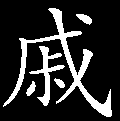
\includegraphics[width=3mm]{../Images/00005}彩笔辉光若转环,心情魔态几千般。写成浓淡兼深浅,活现痴人恋恋间。}

{  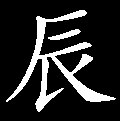
\includegraphics[width=3mm]{../Images/00009}此回写出宝玉闲闯书房偷看袭人,笔意随机跳脱。复又袭人将欲赎身,揣情讽谏,以及宝玉在黛玉房中寻香嘲笑,文字新奇,传奇之中殊所罕见。原本评注过多,未免旁杂,反扰正文。今删去,以俟后之观者凝思入妙,愈显作者之灵机耳。}\href{../Text/part0023_split_000.html\#lnkback_2_a}{\textsuperscript{②}}{}

话说贾妃回宫,次日见驾谢恩,并回奏归省之事,龙颜甚悦,又发内帑彩缎金银等物,以赐贾政及各椒房等员,{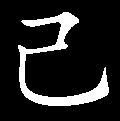
\includegraphics[width=3mm]{../Images/00003}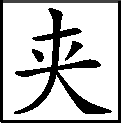
\includegraphics[width=3mm]{../Images/00012}\footnotesize \kaishu 补这一句,细。方见省亲不独贾家一门也。}不必细说。

且说荣宁二府中因连日用尽心力,真是人人力倦,各各神疲,又将园中一应陈设动用之物收拾了两三天方完。第一个凤姐事多任重,别人或可偷安躲静,独他是不能脱得的;二则本性要强,不肯落人褒贬,只扎挣着与无事的人一样。{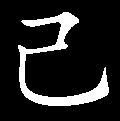
\includegraphics[width=3mm]{../Images/00003}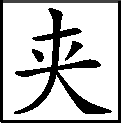
\includegraphics[width=3mm]{../Images/00012}\footnotesize \kaishu 伏下病源。}第一个宝玉是极无事最闲暇的。偏这日一早,袭人的母亲又亲来回过贾母,接袭人家去吃年茶,晚间才得回来。{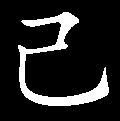
\includegraphics[width=3mm]{../Images/00003}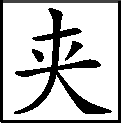
\includegraphics[width=3mm]{../Images/00012}\footnotesize \kaishu 一回一回各生机轴,总在人意想之外。}因此,宝玉只和众丫头们掷骰子赶围棋作戏。{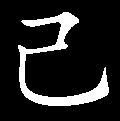
\includegraphics[width=3mm]{../Images/00003}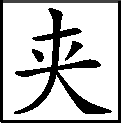
\includegraphics[width=3mm]{../Images/00012}\footnotesize \kaishu 写出正月光景。}正在房内顽的没兴头,忽见丫头们来回说:``东府珍大爷来请过去看戏、放花灯。''宝玉听了,便命换衣裳。才要去时,忽又有贾妃赐出糖蒸酥酪来;{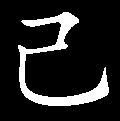
\includegraphics[width=3mm]{../Images/00003}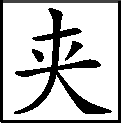
\includegraphics[width=3mm]{../Images/00012}\footnotesize \kaishu 总是新正妙景。}宝玉想上次袭人喜吃此物,便命留与袭人了。自己回过贾母,过去看戏。

谁想贾珍这边唱的是《丁郎认父》、《黄伯央大摆阴魂阵》,更有《孙行者大闹天宫》、《姜子牙斩将封神》等类的戏文。{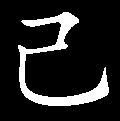
\includegraphics[width=3mm]{../Images/00003}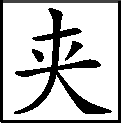
\includegraphics[width=3mm]{../Images/00012}\footnotesize \kaishu 真真热闹。}倏尔神鬼乱出,忽又妖魔毕露,甚至于扬幡过会,号佛行香,锣鼓喊叫之声远闻巷外。{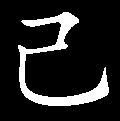
\includegraphics[width=3mm]{../Images/00003}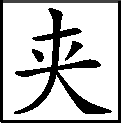
\includegraphics[width=3mm]{../Images/00012}\footnotesize \kaishu 形容刻薄之至,弋阳腔能事毕矣。◇阅至此则有如耳内喧哗、目中撩乱。后文至隔墙闻``袅晴丝''数曲,则有如魂随笛转、魄逐歌销。形容一事,一事毕真,石头是第一能手矣。}满街之人个个都赞:``好热闹戏,别人家断不能有的。''{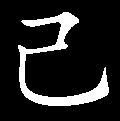
\includegraphics[width=3mm]{../Images/00003}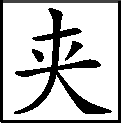
\includegraphics[width=3mm]{../Images/00012}\footnotesize \kaishu 必有之言。}宝玉见繁华热闹到如此不堪的田地,只略坐了一坐,便走开各处闲耍。先是进内去和尤氏和丫鬟姬妾说笑了一回,便出二门来。尤氏等仍料他出来看戏,遂也不曾照管。贾珍、贾琏、薛蟠等只顾猜枚行令,百般作乐,也不理论,纵一时不见他在座,只道在里边去了,故也不问。至于跟宝玉的小厮们,那年纪大些的,知宝玉这一来了,必是晚间才散,因此偷空也有去会赌的,也有往亲友家去吃年茶的,更有或嫖或饮的,都私散了,待晚间再来;那小些的,都钻进戏房里瞧热闹去了。

宝玉见一个人没有,因想``这里素日有个小书房,名\ldots{}\ldots{},内曾挂着一轴美人,极画的得神。今日这般热闹,想那里自然冷静,那美人也自然是寂寞的,须得我去望慰他一回。''{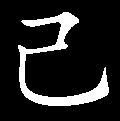
\includegraphics[width=3mm]{../Images/00003}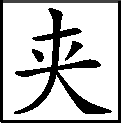
\includegraphics[width=3mm]{../Images/00012}\footnotesize \kaishu 极不通极胡说中写出绝代情痴,宜乎众人谓之疯傻。 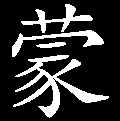
\includegraphics[width=3mm]{../Images/00006}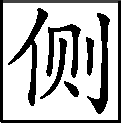
\includegraphics[width=3mm]{../Images/00011}\footnotesize \kaishu 天生一段痴情,所谓``情不情''也。}想着,便往书房里来。刚到窗前,闻得房内有呻吟之韵。宝玉倒唬了一跳:敢是美人活了不成?{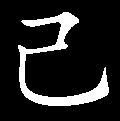
\includegraphics[width=3mm]{../Images/00003}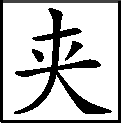
\includegraphics[width=3mm]{../Images/00012}\footnotesize \kaishu 又带出小儿心意,一丝不落。}乃乍着胆子,舔破窗纸,向内一看,那轴美人却不曾活,却是茗烟按着一个女孩子,也干那警幻所训之事。宝玉禁不住大叫:``了不得!''一脚踹进门去,将那两个唬开了,抖衣而颤。

茗烟见是宝玉,忙跪求不迭。宝玉道:``青天白日,这是怎么说。{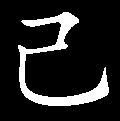
\includegraphics[width=3mm]{../Images/00003}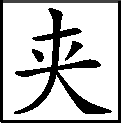
\includegraphics[width=3mm]{../Images/00012}\footnotesize \kaishu 开口便好。}珍大爷知道,你是死是活?''一面看那丫头,虽不标致,倒还白净,些微亦有动人处,羞的面红耳赤,低首无言。宝玉跺脚道:``还不快跑!''{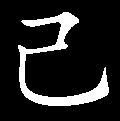
\includegraphics[width=3mm]{../Images/00003}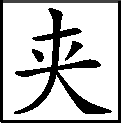
\includegraphics[width=3mm]{../Images/00012}\footnotesize \kaishu 此等搜神夺魄、至神至妙处,只在囫囵不解中得。}一语提醒了那丫头,飞也似去了。宝玉又赶出去叫道:``你别怕,我是不告诉人的。''{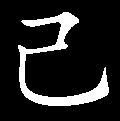
\includegraphics[width=3mm]{../Images/00003}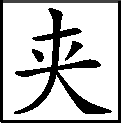
\includegraphics[width=3mm]{../Images/00012}\footnotesize \kaishu 活宝玉,移之他人不可。}急的茗烟在后叫:``祖宗,这是分明告诉人了!''宝玉因问:``那丫头十几岁了?''茗烟道:``大不过十六七岁了。''宝玉道:``连他的岁属也不问问,别的自然越发不知了。可见他白认得你了。可怜,可怜!''{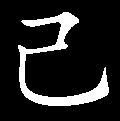
\includegraphics[width=3mm]{../Images/00003}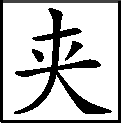
\includegraphics[width=3mm]{../Images/00012}\footnotesize \kaishu 按此书中写一宝玉,其宝玉之为人,是我辈于书中见而知有此人,实未目曾亲睹者。又写宝玉之发言,每每令人不解;宝玉之生性,件件令人可笑;不独于世上亲见这样的人不曾,即阅今古所有之小说传奇中,亦未见这样的文字。于颦儿处更为甚。其囫囵不解之中实可解,可解之中又说不出理路。合目思之,却如真见一宝玉,真闻此言者,移至第二人万不可,亦不成文字矣。余阅《石头记》中至奇至妙之文,全在宝玉颦儿至痴至呆、囫囵不解之语中,其诗词、雅谜、酒令、奇衣、奇食、奇玩等类固他书中未能,然在此书中评之,犹为二着。}又问:``名字叫什么?''茗烟大笑道:``若说出名字来话长,真真新鲜奇文,\href{../Text/part0023_split_000.html\#lnkback_3_a}{\textsuperscript{③}}竟是写不出来的。{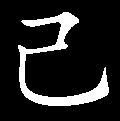
\includegraphics[width=3mm]{../Images/00003}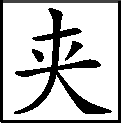
\includegraphics[width=3mm]{../Images/00012}\footnotesize \kaishu 若都写的出来,何以见此书中之妙?脂砚。}据他说,他母亲养他的时节做了梦,{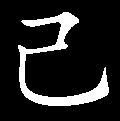
\includegraphics[width=3mm]{../Images/00003}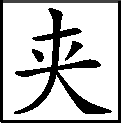
\includegraphics[width=3mm]{../Images/00012}\footnotesize \kaishu 又一个梦,只是随手成趣耳。}梦见得了一匹锦,上面是五色富贵不断头卍字的花样,{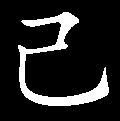
\includegraphics[width=3mm]{../Images/00003}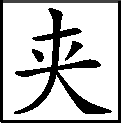
\includegraphics[width=3mm]{../Images/00012}\footnotesize \kaishu 千奇百怪之想。所谓``牛溲马渤皆至药也,鱼鸟昆虫皆妙文也'',天地间无一物不是妙物,无一物不可不成文,但在人意拾取耳。此皆信手拈来随笔成趣,大游戏、大慧悟、大解脱之妙文也。}所以他的名字叫作卍儿。''{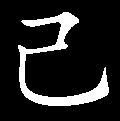
\includegraphics[width=3mm]{../Images/00003}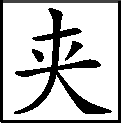
\includegraphics[width=3mm]{../Images/00012}\footnotesize \kaishu 音万。}宝玉听了笑道:``真也新奇,想必他将来有些造化。''说着,沉思一会。

茗烟因问:``二爷为何不看这样的好戏?''宝玉道:``看了半日,怪烦的,出来逛逛,就遇见你们了。这会子作什么呢?''茗烟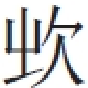
\includegraphics[width=4mm]{../images/00025}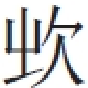
\includegraphics[width=4mm]{../images/00025}\href{../Text/part0023_split_000.html\#lnkback_4_a}{\textsuperscript{④}}{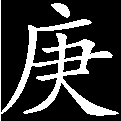
\includegraphics[width=3mm]{../Images/00004}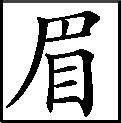
\includegraphics[width=3mm]{../Images/00010}\footnotesize \kaishu 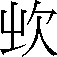
\includegraphics[width=
3mm]{../images/00026},音希。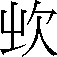
\includegraphics[width=3mm]{../images/00026}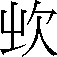
\includegraphics[width=3mm]{../images/00026},笑貌。}笑道:``这会子没人知道,我悄悄的引二爷往城外逛逛去,一会子再往这里来,他们就不知道了。''{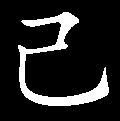
\includegraphics[width=3mm]{../Images/00003}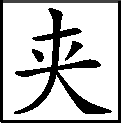
\includegraphics[width=3mm]{../Images/00012}\footnotesize \kaishu 茗烟此时只要掩饰方才之过,故设此以悦宝玉之心。}宝玉道:``不好,仔细花子拐了去。便是他们知道了,又闹大了,不如往熟近些的地方去,还可就来。''茗烟道:``熟近地方,谁家可去?这却难了。''宝玉笑道:``依我的主意,咱们竟找你花大姐姐去,瞧他在家作什么呢。''{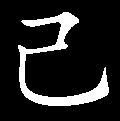
\includegraphics[width=3mm]{../Images/00003}\includegraphics[width=3mm]{../Images/00012}\footnotesize \kaishu 妙!宝玉心中早安了这着,但恐茗烟不肯引去耳。恰遇茗烟私行淫媾,为宝玉所胁,故以城外引以悦其心,宝玉始说出往花家去。非茗烟适有罪所胁,万不敢如此私引出外。别家子弟尚不敢私出,况宝玉哉?况茗烟哉?文字榫楔,细极!}茗烟笑道:``好,好!倒忘了他家。''又道:``若他们知道了,说我引着二爷胡走,要打我呢?''{\includegraphics[width=3mm]{../Images/00003}\includegraphics[width=3mm]{../Images/00012}\footnotesize \kaishu 必不可少之语。}宝玉笑道:``有我呢。''茗烟听说,拉了马,二人从后门就走了。

幸而袭人家不远,不过一半里路程,展眼已到门前。茗烟先进去,叫袭人之兄花自芳。{\includegraphics[width=3mm]{../Images/00003}\includegraphics[width=3mm]{../Images/00012}\footnotesize \kaishu 随姓成名,随手成文。}彼时袭人之母接了袭人与几个外甥女儿、{\includegraphics[width=3mm]{../Images/00003}\includegraphics[width=3mm]{../Images/00012}\footnotesize \kaishu 一树千枝,一源万派,无意随手,伏脉千里。}几个侄女儿来家,正吃果茶。听见外面有人叫``花大哥'',花自芳忙出去看时,见是他主仆两个,唬的惊疑不止,连忙抱下宝玉来,在院内嚷道:``宝二爷来了!''别人听见还可,袭人听了,也不知为何,忙跑出来迎着宝玉,一把拉着问:``你怎么来了?''宝玉笑道:``我怪闷的,来瞧瞧你作什么呢。''袭人听了,才放下心来,{\includegraphics[width=3mm]{../Images/00003}\includegraphics[width=3mm]{../Images/00012}\footnotesize \kaishu 精细周到。}``嗐''了一声,笑{\includegraphics[width=3mm]{../Images/00003}\includegraphics[width=3mm]{../Images/00012}\footnotesize \kaishu 转至``笑''字,妙,神!}道:``你也忒胡闹了,{\includegraphics[width=3mm]{../Images/00003}\includegraphics[width=3mm]{../Images/00012}\footnotesize \kaishu 该说,说得是。}可作什么来呢!''一面又问茗烟:``还有谁跟来?''{\includegraphics[width=3mm]{../Images/00003}\includegraphics[width=3mm]{../Images/00012}\footnotesize \kaishu 细。}茗烟笑道:``别人都不知,就只我们两个。''袭人听了,复又惊慌,{\includegraphics[width=3mm]{../Images/00003}\includegraphics[width=3mm]{../Images/00012}\footnotesize \kaishu 是必有之神理,非特故作顿挫。}说道:``这还了得!倘或碰见了人,或是遇见了老爷,街上人挤车碰,马轿纷纷的,若有个闪失,也是顽得的!你们的胆子比斗还大。都是茗烟调唆的,回去我定告诉嬷嬷们打你。''{\includegraphics[width=3mm]{../Images/00003}\includegraphics[width=3mm]{../Images/00012}\footnotesize \kaishu 该说,说的更是。脂砚。}茗烟撅了嘴道:``二爷骂着打着,叫我引了来,这会子推到我身上。我说别来罢,不然我们还去罢。''{\includegraphics[width=3mm]{../Images/00003}\includegraphics[width=3mm]{../Images/00012}\footnotesize \kaishu 茗烟贼。}花自芳忙劝:``罢了,已是来了,也不用多说了。只是茅檐草舍,又窄又脏,爷怎么坐呢?''

袭人之母也早迎了出来。袭人拉了宝玉进去。宝玉见房中三五个女孩儿,见他进来,都低了头,羞惭惭的。花自芳母子两个百般怕宝玉冷,又让他上炕,又忙另摆果桌,又忙倒好茶。{\includegraphics[width=3mm]{../Images/00003}\includegraphics[width=3mm]{../Images/00012}\footnotesize \kaishu 连用三``又''字,上文一个``百般'',神理活现。脂砚。}袭人笑道:``你们不用白忙,{\includegraphics[width=3mm]{../Images/00003}\includegraphics[width=3mm]{../Images/00012}\footnotesize \kaishu 妙!不写袭卿忙,正是忙之至。若一写袭人忙,便是庸俗小派了。}我自然知道。果子也不用摆,也不敢乱给东西吃。''{\includegraphics[width=3mm]{../Images/00003}\includegraphics[width=3mm]{../Images/00012}\footnotesize \kaishu 如此至微至小中便带出{[}世{]}家常情,他书写不及此。 \includegraphics[width=3mm]{../Images/00006}\includegraphics[width=3mm]{../Images/00011}\footnotesize \kaishu 至敬至情。}一面说,一面将自己的坐褥拿了铺在一个杌子上,宝玉坐了;用自己的脚炉垫了脚,向荷包内取出两个梅花香饼儿来,又将自己的手炉掀开焚上,仍盖好,放与宝玉怀内;然后将自己的茶杯斟了茶,送与宝玉。{\includegraphics[width=3mm]{../Images/00003}\includegraphics[width=3mm]{../Images/00012}\footnotesize \kaishu 叠用四``自己''字,写得宝袭二人素日如何亲洽,如何尊荣,此时一盘托出。盖素日身居侯府绮罗锦绣之中,其安富尊荣之宝玉,亲密浃洽、勤慎委婉之袭人,是分所应当不必写者也。今于此一补,更见其二人平素之情义,且暗透此回中所有母女兄长欲为赎身角口等未到之过文。}彼时他母兄已是忙另齐齐整整摆上一桌子果品来。袭人见总无可吃之物,{{\includegraphics[width=3mm]{../Images/00003}\includegraphics[width=3mm]{../Images/00012}\footnotesize \kaishu 补明宝玉自幼何等娇贵。以此一句留与下部后数十回``寒冬噎酸}虀{,雪夜围破毡''等处对看,可为后生过分之戒。叹叹!}}因笑道:``既来了,没有空去之理,好歹尝一点儿,也是来我家一趟。''{\includegraphics[width=3mm]{../Images/00003}\includegraphics[width=3mm]{../Images/00012}\footnotesize \kaishu 得意之态,是才与母兄较争以后之神理。最细。}说着,便拈了几个松子穰,{\includegraphics[width=3mm]{../Images/00003}\includegraphics[width=3mm]{../Images/00012}\footnotesize \kaishu 唯此品稍可一拈,别品便大错了。}吹去细皮,用手帕托着送与宝玉。

宝玉看见袭人两眼微红,粉光融滑,{\includegraphics[width=3mm]{../Images/00003}\includegraphics[width=3mm]{../Images/00012}\footnotesize \kaishu 八字画出才收泪之一女儿,是好形容,且是宝玉眼中意中。}因悄问袭人:``好好的哭什么?''袭人笑道:``何尝哭,才迷了眼揉的。''因此便遮掩过了。{\includegraphics[width=3mm]{../Images/00003}\includegraphics[width=3mm]{../Images/00012}\footnotesize \kaishu 伏下后文所补未到多少文字。}当下宝玉穿着大红金蟒狐腋箭袖,外罩石青貂裘排穗褂。袭人道:``你特为往这里来又换新服,他们{\includegraphics[width=3mm]{../Images/00003}\includegraphics[width=3mm]{../Images/00012}\footnotesize \kaishu 指晴雯麝月等。}就不问你往那去的?''{\includegraphics[width=3mm]{../Images/00003}\includegraphics[width=3mm]{../Images/00012}\footnotesize \kaishu 必有是问。◇阅此则又笑尽小说中无故家常穿红挂绿、绮绣绫罗等语,自谓是富贵语,究竟反是寒酸话。}宝玉笑道:``珍大哥请过去看戏换的。''袭人点头。又道:``坐一坐就回去罢,这个地方不是你来的。''宝玉笑道:``你就家去才好呢,我还替你留着好东西呢。''{\includegraphics[width=3mm]{../Images/00004}\includegraphics[width=3mm]{../Images/00011}\footnotesize \kaishu ``生员切己之事}\href{../Text/part0023_split_000.html\#lnkback_5_a}{\textsuperscript{⑤}}{''。}袭人悄笑道:``悄悄的,叫他们听着什么意思。''{\includegraphics[width=3mm]{../Images/00003}\includegraphics[width=3mm]{../Images/00012}\footnotesize \kaishu 想见二人素日情常。 \includegraphics[width=3mm]{../Images/00006}\includegraphics[width=3mm]{../Images/00011}\footnotesize \kaishu 追魂。}一面又伸手从宝玉项上将通灵玉摘了下来,向他姊妹们笑道:``你们见识见识。时常说起来都当希罕,{\includegraphics[width=3mm]{../Images/00006}\includegraphics[width=3mm]{../Images/00011}\footnotesize \kaishu 不可少之文。}恨不能一见,今儿可尽力瞧了。再瞧什么希罕物儿,也不过是这么个东西。''{\includegraphics[width=3mm]{../Images/00003}\includegraphics[width=3mm]{../Images/00012}\footnotesize \kaishu 行文至此,固好看之极,且勿论。按此言固是袭人得意之语,盖言你等所稀罕不得一见之宝,我却常守常见,视为平物。然余今窥其用意之旨,则是作者借此,正为贬玉原非大观者也。}说毕,递与他们传看了一遍,仍与宝玉挂好。{\includegraphics[width=3mm]{../Images/00004}\includegraphics[width=3mm]{../Images/00010}\footnotesize \kaishu 自``一把拉住''至此诸形景动作,袭卿有意微露绛芸轩中隐事也。}又命他哥哥去或雇一乘小轿,或雇一辆小车,送宝玉回去。花自芳道:``有我送去,骑马也不妨了。''{\includegraphics[width=3mm]{../Images/00004}\includegraphics[width=3mm]{../Images/00011}\footnotesize \kaishu 只知保重耳。}袭人道:``不为不妨,为的是碰见人。''{\includegraphics[width=3mm]{../Images/00003}\includegraphics[width=3mm]{../Images/00012}\footnotesize \kaishu 细极!}

花自芳忙去雇了一顶小轿来,众人也不敢相留,只得送宝玉出去。袭人又抓果子与茗烟,又把些钱与他买花炮放,教他:``不可告诉人,连你也有不是。''{\includegraphics[width=3mm]{../Images/00006}\includegraphics[width=3mm]{../Images/00011}\footnotesize \kaishu 细密。}一直送宝玉至门前,看着上轿,放下轿帘。花、茗二人牵马跟随。来至宁府街,茗烟命住轿,向花自芳道:``须等我同二爷还到东府里混一混,才好过去的,不然人家就疑惑了。''花自芳听说有理,忙将宝玉抱出轿来,送上马去。宝玉笑说:``倒难为你了。''{\includegraphics[width=3mm]{../Images/00004}\includegraphics[width=3mm]{../Images/00011}\footnotesize \kaishu 公子口气。}于是仍进后门来。俱不在话下。

却说宝玉自出了门,他房中这些丫鬟们都越性恣意的顽笑,也有赶围棋的,也有掷骰抹牌的,磕了一地瓜子皮。偏奶母李嬷嬷拄拐进来请安,瞧瞧宝玉,见宝玉不在家,丫头们只顾玩闹,十分看不过。{\includegraphics[width=3mm]{../Images/00003}\includegraphics[width=3mm]{../Images/00012}\footnotesize \kaishu 人人都看不过,独宝玉看得过。}因叹道:``只从我出去了,不大进来,你们越发没个样儿了,{\includegraphics[width=3mm]{../Images/00003}\includegraphics[width=3mm]{../Images/00012}\footnotesize \kaishu 说得是,原该说。}别的妈妈们越不敢说你们了。{\includegraphics[width=3mm]{../Images/00003}\includegraphics[width=3mm]{../Images/00012}\footnotesize \kaishu 补明好!宝玉虽不吃乳,岂无伴从之媪妪哉?}那宝玉是个丈八的灯台------照见人家,照不见自家的。{\includegraphics[width=3mm]{../Images/00003}\includegraphics[width=3mm]{../Images/00012}\footnotesize \kaishu 用俗语入,妙!}只知嫌人家脏,这是他的屋子,由着你们糟蹋,越不成体统了。''{\includegraphics[width=3mm]{../Images/00003}\includegraphics[width=3mm]{../Images/00012}\footnotesize \kaishu 所以为今古未有之一宝玉。}这些丫头们明知宝玉不讲究这些,二则李嬷嬷已是告老解事出去的了,{\includegraphics[width=3mm]{../Images/00003}\includegraphics[width=3mm]{../Images/00012}\footnotesize \kaishu 调侃入微,妙妙!}如今管他们不着。因此只顾顽,并不理他。那李嬷嬷还只管问``宝玉如今一顿吃多少饭''、``什么时辰睡觉''等语。{\includegraphics[width=3mm]{../Images/00003}\includegraphics[width=3mm]{../Images/00012}\footnotesize \kaishu 可叹!}丫头们总胡乱答应。有的说:``好一个讨厌的老货!''{{\includegraphics[width=3mm]{../Images/00004}\includegraphics[width=3mm]{../Images/00011}\footnotesize \kaishu 实在有的。 }\includegraphics[width=3mm]{../Images/00006}\includegraphics[width=3mm]{../Images/00011}\footnotesize \kaishu 入神。}

李嬷嬷又问道:``这盖碗里是酥酪,怎不送与我去?我就吃了罢。''说毕,拿匙就吃。{\includegraphics[width=3mm]{../Images/00003}\includegraphics[width=3mm]{../Images/00012}\footnotesize \kaishu 写龙钟奶母,便是龙钟奶母。}一个丫头道:``快别动!那是说了给袭人留着的,{\includegraphics[width=3mm]{../Images/00003}\includegraphics[width=3mm]{../Images/00012}\footnotesize \kaishu 过下无痕。}回来又惹气了。{\includegraphics[width=3mm]{../Images/00003}\includegraphics[width=3mm]{../Images/00012}\footnotesize \kaishu 照应茜雪枫露茶前案。}你老人家自己承认,别带累我们受气。''{\includegraphics[width=3mm]{../Images/00003}\includegraphics[width=3mm]{../Images/00012}\footnotesize \kaishu 这等话语声口,必是晴雯无疑。}李嬷嬷听了,又气又愧,便说道:``我不信他这样坏了。别说我吃了一碗牛奶,就是再比这个值钱的,也是应该的。难道待袭人比我还重?难道他不想想怎么长大了?我的血变的奶,吃的长这么大,如今我吃他一碗牛奶,他就生气了?我偏吃了,看怎么样!你们看袭人不知怎样,那是我手里调理出来的毛丫头,什么阿物儿!''{\includegraphics[width=3mm]{../Images/00003}\includegraphics[width=3mm]{../Images/00012}\footnotesize \kaishu 虽暂委屈唐突袭卿,然亦怨不得李媪。}一面说,一面赌气将酥酪吃尽。又一丫头笑道:``他们不会说话,怨不得你老人家生气。宝玉还时常送东西孝敬你老去,岂有为这个不自在的。''{\includegraphics[width=3mm]{../Images/00003}\includegraphics[width=3mm]{../Images/00012}\footnotesize \kaishu 听这声口,必是麝月无疑。}李嬷嬷道:``你们也不必妆狐媚子哄我,打量上次为茶撵茜雪的事我不知道呢。{\includegraphics[width=3mm]{../Images/00003}\includegraphics[width=3mm]{../Images/00012}\footnotesize \kaishu 照应前文,又用一``撵'',屈杀宝玉,然李媪心中口中毕肖。}明儿有了不是,我再来领!''说着,赌气去了。{\includegraphics[width=3mm]{../Images/00003}\includegraphics[width=3mm]{../Images/00012}\footnotesize \kaishu 过至下回。}

少时,宝玉回来,命人去接袭人。只见晴雯躺在床上不动,{\includegraphics[width=3mm]{../Images/00003}\includegraphics[width=3mm]{../Images/00012}\footnotesize \kaishu 娇态已惯。}宝玉因问:``敢是病了?再不然输了?''秋纹道:``他倒是赢的。谁知李老太太来了,混输了,他气的睡去了。''宝玉笑道:``你别和他一般见识,由他去就是了。''说着,袭人已来,彼此相见。袭人又问宝玉何处吃饭,多早晚回来,又代母妹问诸同伴姊妹好。一时换衣卸妆。宝玉命取酥酪来,丫鬟们回说:``李奶奶吃了。''宝玉才要说话,袭人便忙笑说道:``原来是留的这个,多谢费心。前儿我吃的时候好吃,吃过了好肚子疼,足的吐了才好。他吃了倒好,搁在这里倒白糟蹋了。{\includegraphics[width=3mm]{../Images/00003}\includegraphics[width=3mm]{../Images/00012}\footnotesize \kaishu 与前文应失手碎钟遥对,通部袭人皆是如此,一丝不错。}我只想风干栗子吃,你替我剥栗子,我去铺炕。''{\includegraphics[width=3mm]{../Images/00003}\includegraphics[width=3mm]{../Images/00012}\footnotesize \kaishu 必如此方是。}

宝玉听了信以为真,方把酥酪丢开,取栗子来,自向灯前检剥。一面见众人不在房中,乃笑问袭人道:``今儿那个穿红的是你什么人?''{\includegraphics[width=3mm]{../Images/00003}\includegraphics[width=3mm]{../Images/00012}\footnotesize \kaishu 若是见过女儿之后没有一段文字,便不是宝玉,亦非《石头记》矣。}袭人道:``那是我两姨妹子。''宝玉听了,赞叹了两声。{\includegraphics[width=3mm]{../Images/00003}\includegraphics[width=3mm]{../Images/00012}\footnotesize \kaishu 这一赞叹又是令人囫囵不解之语,只此便抵过一大篇文字。}袭人道:``叹什么?{\includegraphics[width=3mm]{../Images/00003}\includegraphics[width=3mm]{../Images/00012}\footnotesize \kaishu 只一``叹''字,便引出``花解语''一回来。}我知道你心里的缘故,想是说他那里配红的。''{\includegraphics[width=3mm]{../Images/00003}\includegraphics[width=3mm]{../Images/00012}\footnotesize \kaishu 补出宝玉素喜红色,这是激语。}宝玉笑道:``不是,不是。那样的不配穿红的,谁还敢穿。{\includegraphics[width=3mm]{../Images/00003}\includegraphics[width=3mm]{../Images/00012}\footnotesize \kaishu 活宝玉。}我因为见他实在好的很,怎么也得他在咱们家就好了。''{\includegraphics[width=3mm]{../Images/00003}\includegraphics[width=3mm]{../Images/00012}\footnotesize \kaishu 妙谈妙意。}袭人冷笑道:``我一个人是奴才命罢了,难道连我的亲戚都是奴才命不成?定还要拣实在好的丫头才往你家来?''{\includegraphics[width=3mm]{../Images/00003}\includegraphics[width=3mm]{../Images/00012}\footnotesize \kaishu 妙答。宝玉并未说``奴才''二字,袭人连补``奴才''二字最是劲节,怨不得作此语。}宝玉听了,忙笑道:``你又多心了。我说往咱们家来,必定是奴才不成?{\includegraphics[width=3mm]{../Images/00003}\includegraphics[width=3mm]{../Images/00012}\footnotesize \kaishu 勉强,如闻。}说亲戚就使不得?''{\includegraphics[width=3mm]{../Images/00003}\includegraphics[width=3mm]{../Images/00012}\footnotesize \kaishu 更勉强。 \includegraphics[width=3mm]{../Images/00006}\includegraphics[width=3mm]{../Images/00011}\footnotesize \kaishu 这样妙文,何处得来?非目见身行,岂能如此的确?}袭人道:``那也搬配不上。''{\includegraphics[width=3mm]{../Images/00003}\includegraphics[width=3mm]{../Images/00012}\footnotesize \kaishu 说的是。}宝玉便不肯再说,只是剥栗子。袭人笑道:``怎么不言语了?想是我才冒撞冲犯了你?明儿赌气花几两银子买他们进来就是了。''{\includegraphics[width=3mm]{../Images/00003}\includegraphics[width=3mm]{../Images/00012}\footnotesize \kaishu 总是故意激他。}宝玉笑道:``你说的话,怎么叫我答言呢。我不过是赞他好,正配生在这深堂大院里,没的我们这种浊物{\includegraphics[width=3mm]{../Images/00003}\includegraphics[width=3mm]{../Images/00012}\footnotesize \kaishu 妙号!后文又曰``须眉浊物''之称,今古未有之一人始有此今古未有之妙称妙号。}倒生在这里。''{\includegraphics[width=3mm]{../Images/00003}\includegraphics[width=3mm]{../Images/00012}\footnotesize \kaishu 这皆是宝玉意中心中确实之念,非前勉强之词,所以谓今古未有之一人耳。听其囫囵不解之言,察其幽微感触之心,审其痴妄委婉之意,皆今古未见之人,亦是未见之文字。说不得贤,说不得愚,说不得不肖,说不得善,说不得恶,说不得正大光明,说不得混账恶赖,说不得聪明才俊,说不得庸俗平凡,说不得好色好淫,说不得情痴情种,恰恰只有一颦儿可对,令他人徒加评论,总未摸着他二人是何等脱胎、何等心臆、何等骨肉。余阅此书,亦爱其文字耳,实亦不能评出此二人终是何等人物。后观《情榜》评曰``宝玉情不情'',``黛玉情情'',此二评自在评痴之上,亦属囫囵不解,妙甚!}袭人道:``他虽没这造化,倒也是娇生惯养的呢,我姨爹姨娘的宝贝。如今十七岁,各样的嫁妆都齐备了,明年就出嫁。''{\includegraphics[width=3mm]{../Images/00004}\includegraphics[width=3mm]{../Images/00011}\footnotesize \kaishu 所谓不入耳之言也。}

宝玉听了``出嫁''二字,不禁又嗐了两声。{\includegraphics[width=3mm]{../Images/00003}\includegraphics[width=3mm]{../Images/00012}\footnotesize \kaishu 宝玉心思另是一样,余前评可见。}正不自在,又听袭人叹道:{\includegraphics[width=3mm]{../Images/00003}\includegraphics[width=3mm]{../Images/00012}\footnotesize \kaishu 袭人亦叹,自有别论。}``只从我来这几年,姊妹们都不得在一处。如今我要回去了,他们又都去了。''宝玉听这话内有文章,{\includegraphics[width=3mm]{../Images/00003}\includegraphics[width=3mm]{../Images/00012}\footnotesize \kaishu 余亦如此。}不觉吃一惊,{\includegraphics[width=3mm]{../Images/00003}\includegraphics[width=3mm]{../Images/00012}\footnotesize \kaishu 余亦吃惊。}忙丢下栗子,问道:``怎么,你如今要回去了?''袭人道:``我今儿听见我妈和哥哥商议,教我再耐烦一年,明年他们上来,就赎我出去的呢。''{\includegraphics[width=3mm]{../Images/00003}\includegraphics[width=3mm]{../Images/00012}\footnotesize \kaishu 即余今日犹难为情,况当日之宝玉哉?}宝玉听了这话,越发怔了,因问:``为什么要赎你?''袭人道:``这话奇了!我又比不得是你这里的家生子儿,一家子都在别处,独我一个人在这里,怎么是个了局?''{\includegraphics[width=3mm]{../Images/00003}\includegraphics[width=3mm]{../Images/00012}\footnotesize \kaishu 说得极是。}宝玉道:``我不叫你去也难。''{\includegraphics[width=3mm]{../Images/00003}\includegraphics[width=3mm]{../Images/00012}\footnotesize \kaishu 是头一句驳,故用贵公子声口,无理。}袭人道:``从来没这道理。便是朝廷宫里,也有个定例,或几年一选,几年一入,也没有个长远留下人的理,别说你了!''{\includegraphics[width=3mm]{../Images/00003}\includegraphics[width=3mm]{../Images/00012}\footnotesize \kaishu 一驳,更有理。}

宝玉想一想,果然有理。{\includegraphics[width=3mm]{../Images/00003}\includegraphics[width=3mm]{../Images/00012}\footnotesize \kaishu 自然。}又道:``老太太不放你也难。''{\includegraphics[width=3mm]{../Images/00003}\includegraphics[width=3mm]{../Images/00012}\footnotesize \kaishu 第二层仗祖母溺爱,更无理。}袭人道:``为什么不放?我果然是个最难得的,或者感动了老太太、太太,{\includegraphics[width=3mm]{../Images/00003}\includegraphics[width=3mm]{../Images/00012}\footnotesize \kaishu 宝玉并不提王夫人,袭人偏自补出,周密之至!}必不放我出去的,设或多给我们家几两银子,留下我,容或有之;其实我也不过是个平常的人,{\includegraphics[width=3mm]{../Images/00006}\includegraphics[width=3mm]{../Images/00011}\footnotesize \kaishu 此等语言便是袭卿心事。}比我强的多而且多。自我从小儿来了,跟着老太太,先伏侍了史大姑娘几年,{\includegraphics[width=3mm]{../Images/00003}\includegraphics[width=3mm]{../Images/00012}\footnotesize \kaishu 百忙中又补出湘云来,真是七穿八达,得空便入。}如今又伏侍了你几年。如今我们家来赎,正是该叫去的,只怕连身价也不要,就开恩叫我去呢。若说为伏侍的你好,不叫我去,断然没有的事。那伏侍的好,是分内应当的,{\includegraphics[width=3mm]{../Images/00004}\includegraphics[width=3mm]{../Images/00011}\footnotesize \kaishu 这却是真心话。}不是什么奇功。我去了,仍旧有好的来了,不是没了我就不成事。''{\includegraphics[width=3mm]{../Images/00003}\includegraphics[width=3mm]{../Images/00012}\footnotesize \kaishu 再一驳,更精细,更有理。 \includegraphics[width=3mm]{../Images/00006}\includegraphics[width=3mm]{../Images/00011}\footnotesize \kaishu 反敲。}宝玉听了这些话,竟是有去的理,无留的理,{\includegraphics[width=3mm]{../Images/00003}\includegraphics[width=3mm]{../Images/00012}\footnotesize \kaishu 自然。}心内越发急了,{\includegraphics[width=3mm]{../Images/00003}\includegraphics[width=3mm]{../Images/00012}\footnotesize \kaishu 原当急。}因又道:``虽然如此说,我只一心留下你,不怕老太太不和你母亲说。多多给你母亲些银子,他也不好意思接你了。''{\includegraphics[width=3mm]{../Images/00003}\includegraphics[width=3mm]{../Images/00012}\footnotesize \kaishu 急心肠,故入于霸道。无理。 \includegraphics[width=3mm]{../Images/00006}\includegraphics[width=3mm]{../Images/00011}\footnotesize \kaishu 三字入神。}袭人道:``我妈自然不敢强。且漫说和他好说,又多给银子;就便不和他好说,一个钱也不给,安心要强留下我,他也不敢不依。但只是咱们家从没干过这倚势仗贵霸道的事。这比不得别的东西,因为你喜欢,加十倍利弄了来给你,那卖的人不得吃亏,可以行得。如今无故平空留下我,于你又无益,反叫我们骨肉分离,这件事,老太太、太太断不肯行的。''{\includegraphics[width=3mm]{../Images/00003}\includegraphics[width=3mm]{../Images/00012}\footnotesize \kaishu 三驳,不独更有理,且又补出贾府自家慈善宽厚等事。}宝玉听了,思忖半晌,{\includegraphics[width=3mm]{../Images/00003}\includegraphics[width=3mm]{../Images/00012}\footnotesize \kaishu 正是思忖只有去理,实无留理。}乃说道:``依你说,你是去定了?''{\includegraphics[width=3mm]{../Images/00003}\includegraphics[width=3mm]{../Images/00012}\footnotesize \kaishu 自然。}袭人道:``去定了。''{\includegraphics[width=3mm]{../Images/00004}\includegraphics[width=3mm]{../Images/00011}\footnotesize \kaishu 口气像极。}宝玉听了,自思道:``谁知这样一个人,这样薄情无义。''{\includegraphics[width=3mm]{../Images/00003}\includegraphics[width=3mm]{../Images/00012}\footnotesize \kaishu 余亦如此见疑。}乃叹道:``早知道都是要去的,{\includegraphics[width=3mm]{../Images/00003}\includegraphics[width=3mm]{../Images/00012}\footnotesize \kaishu ``都是要去的'',妙!可谓触类旁通,活是宝玉。 \includegraphics[width=3mm]{../Images/00006}\includegraphics[width=3mm]{../Images/00011}\footnotesize \kaishu 上古至今及后世有情者,同声一哭!}我就不该弄了来,临了剩了我一个孤鬼儿。''{\includegraphics[width=3mm]{../Images/00003}\includegraphics[width=3mm]{../Images/00012}\footnotesize \kaishu 可谓见首知尾,活是宝玉。}说着,便赌气上床睡去了。{\includegraphics[width=3mm]{../Images/00003}\includegraphics[width=3mm]{../Images/00012}\footnotesize \kaishu 又到无可奈何之时了。}

原来袭人在家,听见他母兄要赎他回去,{\includegraphics[width=3mm]{../Images/00003}\includegraphics[width=3mm]{../Images/00012}\footnotesize \kaishu 补前文。}他就说至死也不回去的。又说:``当日原是你们没饭吃,就剩我还值几两银子,若不叫你们卖,没有个看着老子娘饿死的理。{\includegraphics[width=3mm]{../Images/00003}\includegraphics[width=3mm]{../Images/00012}\footnotesize \kaishu 补出袭人幼时艰辛苦状,与前文之香菱、后文之晴雯大同小异,自是又副十二钗中之冠,故不得不补传之。 {\includegraphics[width=3mm]{../Images/00004}\includegraphics[width=3mm]{../Images/00011}\footnotesize \kaishu 孝女,义女。}}如今幸而卖到这个地方,{\includegraphics[width=3mm]{../Images/00003}\includegraphics[width=3mm]{../Images/00012}\footnotesize \kaishu 可谓不幸中之幸。}吃穿和主子一样,又不朝打暮骂。况且如今爷虽没了,你们却又整理的家成业就,复了元气。若果然还艰难,把我赎出来,再多掏澄几个钱,也还罢了,{\includegraphics[width=3mm]{../Images/00004}\includegraphics[width=3mm]{../Images/00011}\footnotesize \kaishu 孝女,义女。}其实又不难了。这会子又赎我作什么?权当我死了,{\includegraphics[width=3mm]{../Images/00004}\includegraphics[width=3mm]{../Images/00011}\footnotesize \kaishu 可怜可怜!}再不必起赎我的念头!''{\includegraphics[width=3mm]{../Images/00006}\includegraphics[width=3mm]{../Images/00011}\footnotesize \kaishu 同心同志,更觉幸遇。}因此哭闹{\includegraphics[width=3mm]{../Images/00004}\includegraphics[width=3mm]{../Images/00011}\footnotesize \kaishu 我也要哭。}了一阵。{\includegraphics[width=3mm]{../Images/00003}\includegraphics[width=3mm]{../Images/00012}\footnotesize \kaishu 以上补在家今日之事,与宝玉问哭一句针对。}

他母兄见他这般坚执,自然必不出来的了。况且原是卖倒的死契,明仗着贾宅是慈善宽厚之家,不过求一求,只怕身价银一并赏了,这是有的事呢。{\includegraphics[width=3mm]{../Images/00003}\includegraphics[width=3mm]{../Images/00012}\footnotesize \kaishu 又夹带出贾府平素施为来,与袭人口中针对。}二则,贾府中从不曾作践下人,只有恩多威少的。{\includegraphics[width=3mm]{../Images/00003}\includegraphics[width=3mm]{../Images/00012}\footnotesize \kaishu 伏下多少后文。 \includegraphics[width=3mm]{../Images/00006}\includegraphics[width=3mm]{../Images/00011}\footnotesize \kaishu 铁槛寺凤卿受赂,令人怅恨。}且凡老少房中所有亲侍的女孩子们,更比待家下众人不同,平常寒薄人家的小姐,也不能那样尊重的。{\includegraphics[width=3mm]{../Images/00003}\includegraphics[width=3mm]{../Images/00012}\footnotesize \kaishu 又伏下多少后文。先一句是传中陪客,此一句是传中本旨。}因此,他母子两个也就死心不赎了。{\includegraphics[width=3mm]{../Images/00003}\includegraphics[width=3mm]{../Images/00012}\footnotesize \kaishu 既如此,何得袭人又作前语以愚宝玉?不知何意,且看后文。}次后忽然宝玉去了,他二个又是那般景况,{\includegraphics[width=3mm]{../Images/00003}\includegraphics[width=3mm]{../Images/00012}\footnotesize \kaishu 一件闲事一句闲文皆无,警甚。}他母子二人心下更明白了,越发石头落了地,而且是意外之想,彼此放心,再无赎念了。{\includegraphics[width=3mm]{../Images/00003}\includegraphics[width=3mm]{../Images/00012}\footnotesize \kaishu 一段情结。脂砚。}

如今且说袭人自幼见宝玉性格异常,{\includegraphics[width=3mm]{../Images/00003}\includegraphics[width=3mm]{../Images/00012}\footnotesize \kaishu 四字好!所谓``说不得好,又说不得不好''也。}其淘气憨顽自是出于众小儿之外,更有几件千奇百怪口不能言的毛病儿。{\includegraphics[width=3mm]{../Images/00003}\includegraphics[width=3mm]{../Images/00012}\footnotesize \kaishu 只如此说更好。所谓``说不得聪明贤良,说不得痴呆愚昧''也。}近来仗着祖母溺爱,父母亦不能十分严紧拘管,更觉放荡弛纵,{\includegraphics[width=3mm]{../Images/00003}\includegraphics[width=3mm]{../Images/00012}\footnotesize \kaishu 四字妙评。脂砚。}任性恣情,{\includegraphics[width=3mm]{../Images/00003}\includegraphics[width=3mm]{../Images/00012}\footnotesize \kaishu 四字更好。亦不涉于恶,亦不涉于淫,亦不涉于骄,不过一味任性耳。}最不喜务正。{\includegraphics[width=3mm]{../Images/00003}\includegraphics[width=3mm]{../Images/00012}\footnotesize \kaishu 这还是小儿同病。}每欲劝时,料不能听,今日可巧有赎身之论,故先用骗词,以探其情,以压其气,然后好下箴规。{\includegraphics[width=3mm]{../Images/00003}\includegraphics[width=3mm]{../Images/00012}\footnotesize \kaishu 原来如此。 \includegraphics[width=3mm]{../Images/00006}\includegraphics[width=3mm]{../Images/00011}\footnotesize \kaishu 以此法游刃,有何不可解之牛?}今见他默默睡去了,知其情有不忍,气已馁堕。{\includegraphics[width=3mm]{../Images/00003}\includegraphics[width=3mm]{../Images/00012}\footnotesize \kaishu 不独解语,亦且有智。}自己原不想栗子吃的,只因怕为酥酪又生事故,亦如茜雪之茶等事,{\includegraphics[width=3mm]{../Images/00003}\includegraphics[width=3mm]{../Images/00012}\footnotesize \kaishu 可谓贤而多智术之人。}是以假以栗子为由,混过宝玉不提就完了。于是命小丫头子们将栗子拿去吃了,自己来推宝玉。只见宝玉泪痕满面,{\includegraphics[width=3mm]{../Images/00003}\includegraphics[width=3mm]{../Images/00012}\footnotesize \kaishu 正是无可奈何之时。 \includegraphics[width=3mm]{../Images/00006}\includegraphics[width=3mm]{../Images/00011}\footnotesize \kaishu 不知何故,我亦掩涕。}袭人便笑道:``这有什么伤心的,你果然留我,我自然不出去了。''宝玉见这话有文章,{\includegraphics[width=3mm]{../Images/00003}\includegraphics[width=3mm]{../Images/00012}\footnotesize \kaishu 宝玉不愚。}便说道:``你倒说说,我还要怎么留你,我自己也难说了。''{\includegraphics[width=3mm]{../Images/00003}\includegraphics[width=3mm]{../Images/00012}\footnotesize \kaishu 二人素常情义。}袭人笑道:``咱们素日好处,再不用说。但今日你安心留我,不在这上头。我另说出两三件事来,你果然依了我,就是你真心留我了,刀搁在脖子上,我也是不出去的了。''{\includegraphics[width=3mm]{../Images/00006}\includegraphics[width=3mm]{../Images/00011}\footnotesize \kaishu 以此等心,行此等事,昭昭苍天,岂无明见。}

宝玉忙笑道:``你说,那几件?我都依你。好姐姐,好亲姐姐,{\includegraphics[width=3mm]{../Images/00003}\includegraphics[width=3mm]{../Images/00012}\footnotesize \kaishu 叠二语,活见从纸上走一宝玉下来,如闻其呼、如见其笑。}别说两三件,就是两三百件,我也依。{\includegraphics[width=3mm]{../Images/00003}\includegraphics[width=3mm]{../Images/00012}\footnotesize \kaishu ``两三百''不成话,却是宝玉口中。}只求你们同看着我,守着我,等我有一日化成了飞灰,{\includegraphics[width=3mm]{../Images/00003}\includegraphics[width=3mm]{../Images/00012}\footnotesize \kaishu 脂砚斋所谓``不知是何心思,始得口出此等不成话之至奇至妙之话'',诸公请如何解得,如何评论?◇所劝者正为此,偏于劝时一犯,妙甚!}------飞灰还不好,灰还有形有迹,还有知识。{\includegraphics[width=3mm]{../Images/00003}\includegraphics[width=3mm]{../Images/00012}\footnotesize \kaishu 灰还有``知识'',奇之不可胜言矣!余则谓人尚无知识者多多。}等我化成一股轻烟,风一吹便散了的时候,你们也管不得我,我也顾不得你们了。{\includegraphics[width=3mm]{../Images/00006}\includegraphics[width=3mm]{../Images/00011}\footnotesize \kaishu 人人皆以宝玉为痴,孰不知世人比宝玉更痴。}那时凭我去,我也凭你们爱那里去就去了。''{\includegraphics[width=3mm]{../Images/00003}\includegraphics[width=3mm]{../Images/00012}\footnotesize \kaishu 是聪明,是愚昧,是小儿淘气?余皆不知,只觉悲感难言,奇瑰愈妙。}话未说完,急的袭人忙握他的嘴,说:``好好的,正为劝你这些,倒更说的狠了。''宝玉忙说道:``再不说这话了。''{\includegraphics[width=3mm]{../Images/00004}\includegraphics[width=3mm]{../Images/00011}\footnotesize \kaishu 只说今日一次。呵呵,玉兄,玉兄,你到底哄的那一个?}袭人道:``这是头一件要改的。''宝玉道:``改了。再要说,你就拧嘴。还有什么?''

袭人道:``第二件,你真喜读书也罢,假喜也罢,{\includegraphics[width=3mm]{../Images/00004}\includegraphics[width=3mm]{../Images/00011}\footnotesize \kaishu 新鲜,真新鲜!}只是在老爷跟前或在别人跟前,你别只管批驳诮谤,只作出个喜读书的样子来,{\includegraphics[width=3mm]{../Images/00003}\includegraphics[width=3mm]{../Images/00012}\footnotesize \kaishu 宝玉又诮谤读书人?恨此时不能一见如何诮谤。 {\includegraphics[width=3mm]{../Images/00004}\includegraphics[width=3mm]{../Images/00011}\footnotesize \kaishu 所谓``开方便门''。}}也教老爷少生些气,{\includegraphics[width=3mm]{../Images/00004}\includegraphics[width=3mm]{../Images/00011}\footnotesize \kaishu 大家听听,可是丫鬟说的话。}在人前也好说嘴。他心里想着,我家代代读书,只从有了你,不承望你不喜读书,已经他心里又气又愧了。而且背前背后乱说那些混话,凡读书上进的人,你就起个名字叫作`禄蠹';{\includegraphics[width=3mm]{../Images/00003}\includegraphics[width=3mm]{../Images/00012}\footnotesize \kaishu 二字从古未见,新奇之至!难怨世人谓之可杀,余却最喜。}又说只除`明明德'外无书,都是前人自己不能解圣人之书,便另出己意,混编纂出来的。{\includegraphics[width=3mm]{../Images/00003}\includegraphics[width=3mm]{../Images/00012}\footnotesize \kaishu 宝玉目中犹有``明明德''三字,心中犹有``圣人''二字,又素日皆作如是等语,宜乎人人谓之疯傻不肖。}这些话,怎么怨得老爷不气、不时时打你?叫别人怎么想你?''宝玉笑道:``再不说了。那原是那小时不知天高地厚,信口胡说,如今再不敢说了。{\includegraphics[width=3mm]{../Images/00003}\includegraphics[width=3mm]{../Images/00012}\footnotesize \kaishu 又作是语,说不得不乖觉,然又是作者瞒人之处也。}还有什么?''

袭人道:``再不可毁僧谤道,{\includegraphics[width=3mm]{../Images/00003}\includegraphics[width=3mm]{../Images/00012}\footnotesize \kaishu 一件,是妇女心意。}调脂弄粉。{\includegraphics[width=3mm]{../Images/00003}\includegraphics[width=3mm]{../Images/00012}\footnotesize \kaishu 二件,若不如此,亦非宝玉。}还有更要紧的一件,{\includegraphics[width=3mm]{../Images/00003}\includegraphics[width=3mm]{../Images/00012}\footnotesize \kaishu 忽又作此一语。}再不许吃人嘴上擦的胭脂了,{\includegraphics[width=3mm]{../Images/00003}\includegraphics[width=3mm]{../Images/00012}\footnotesize \kaishu 此一句是闻所未闻之语,宜乎其父母严责也。}与那爱红的毛病儿。''宝玉道:``都改,都改。再有什么,快说。''袭人笑道:``再也没有了。只是百事检点些,不任意任情的就是了。{\includegraphics[width=3mm]{../Images/00003}\includegraphics[width=3mm]{../Images/00012}\footnotesize \kaishu 总包括尽矣。其所谓``花解语''者,大矣!不独冗冗为儿女之分也。}你若果都依了,便拿八人轿也抬不出我去了。''宝玉笑道:``你在这里长远了,不怕没八人轿你坐。''袭人冷笑道:``这我可不希罕的。有那个福气,没有那个道理。纵坐了,也没甚趣。''{\includegraphics[width=3mm]{../Images/00003}\includegraphics[width=3mm]{../Images/00012}\footnotesize \kaishu 调侃不浅,然在袭人能作是语,实可爱、可敬、可服之至,所谓``花解语''也。 {\includegraphics[width=3mm]{../Images/00004}\includegraphics[width=3mm]{../Images/00010}\footnotesize \kaishu ``花解语''一段,乃袭卿满心满意将玉兄为终身得靠,千妥万当,故有是{(余)}{[}语{]}。阅至此,余为袭卿一叹。丁亥春。畸笏叟。 }\includegraphics[width=3mm]{../Images/00006}\includegraphics[width=3mm]{../Images/00011}\footnotesize \kaishu 真正逼人。}

二人正说着,只见秋纹走进来,说:``快三更了,该睡了。方才老太太打发嬷嬷来问,我答应睡了。''宝玉命取表来{\includegraphics[width=3mm]{../Images/00003}\includegraphics[width=3mm]{../Images/00012}\footnotesize \kaishu 照应前凤姐之文。}看时,果然针已指到亥正,{\includegraphics[width=3mm]{../Images/00003}\includegraphics[width=3mm]{../Images/00012}\footnotesize \kaishu 表则是表的写法,前形容自鸣钟则是自鸣钟,各尽其神妙。}方从新盥漱,宽衣安歇,不在话下。

至次日清晨,袭人起来,便觉身体发重,头疼目胀,四肢火热。先时还扎挣的住,次后捱不住,只要睡着,因而和衣躺在炕上。{\includegraphics[width=3mm]{../Images/00004}\includegraphics[width=3mm]{../Images/00011}\footnotesize \kaishu 过下引线。}宝玉忙回了贾母,传医诊视,说道:``不过偶感风寒,吃一两剂药疏散疏散就好了。''开方去后,令人取药来煎好,刚服下去,命他盖上被渥汗,宝玉自去黛玉房中来看视。{\includegraphics[width=3mm]{../Images/00003}\includegraphics[width=3mm]{../Images/00012}\footnotesize \kaishu 为下文留地步。}

彼时黛玉自在床上歇午,丫鬟们皆出去自便,满屋内静悄悄的。宝玉揭起绣线软帘,进入里间,只见黛玉睡在那里,忙走上来推他道:``好妹妹,{\includegraphics[width=3mm]{../Images/00003}\includegraphics[width=3mm]{../Images/00012}\footnotesize \kaishu 才住了``好姐姐'',又闻``好妹妹'',大约宝玉一日之中,一时之内,此六个字未曾暂离口角。妙甚!}才吃了饭,又睡觉。''将黛玉唤醒。{\includegraphics[width=3mm]{../Images/00003}\includegraphics[width=3mm]{../Images/00012}\footnotesize \kaishu 若是别部书中写此时之宝玉,一进来便生不轨之心,突萌苟且之念,更有许多贼形鬼状等丑态邪言矣。此却反推唤醒他,毫不在意,所谓``说不得淫荡''是也。}黛玉见是宝玉,因说道:``你且出去逛逛,我前儿闹了一夜,今儿还没有歇过来,{\includegraphics[width=3mm]{../Images/00003}\includegraphics[width=3mm]{../Images/00012}\footnotesize \kaishu 补出娇怯态度。}浑身酸疼。''宝玉道:``酸疼事小,睡出来的病大。我替你解闷儿,混过困去就好了。''{\includegraphics[width=3mm]{../Images/00003}\includegraphics[width=3mm]{../Images/00012}\footnotesize \kaishu 宝玉又知养身。}黛玉只合着眼,说道:``我不困,只略歇歇儿,你且别处去闹会子再来。''宝玉推他道:``我往那里去呢,见了别人就怪腻的。''{\includegraphics[width=3mm]{../Images/00003}\includegraphics[width=3mm]{../Images/00012}\footnotesize \kaishu 所谓只有一颦可对,亦属怪事。}

黛玉听了,``嗤''的一声笑道:``你既要在这里,那边去老老实实的坐着,咱们说话儿。''宝玉道:``我也歪着。''黛玉道:``你就歪着。''宝玉道:``没有枕头,{\includegraphics[width=3mm]{../Images/00003}\includegraphics[width=3mm]{../Images/00012}\footnotesize \kaishu 绵缠密切入微。}咱们在一个枕头上。''{\includegraphics[width=3mm]{../Images/00003}\includegraphics[width=3mm]{../Images/00012}\footnotesize \kaishu 更妙!渐逼渐近,所谓``意绵绵''也。}黛玉道:``放屁!{\includegraphics[width=3mm]{../Images/00004}\includegraphics[width=3mm]{../Images/00011}\footnotesize \kaishu 如闻。}外头不是枕头?拿一个来枕着。''宝玉出至外间,看了一看,回来笑道:``那个我不要,也不知是那个脏婆子的。''黛玉听了,睁开眼,{\includegraphics[width=3mm]{../Images/00003}\includegraphics[width=3mm]{../Images/00012}\footnotesize \kaishu 睁眼。}起身{\includegraphics[width=3mm]{../Images/00003}\includegraphics[width=3mm]{../Images/00012}\footnotesize \kaishu 起身。}笑{\includegraphics[width=3mm]{../Images/00003}\includegraphics[width=3mm]{../Images/00012}\footnotesize \kaishu 笑。}道:``真真你就是我命中的`天魔星'!{\includegraphics[width=3mm]{../Images/00003}\includegraphics[width=3mm]{../Images/00012}\footnotesize \kaishu 妙语,妙之至!想见其态度。}请枕这一个。''说着,将自己枕的推与宝玉,又起身将自己的再拿了一个来,自己枕了,二人对面倒下。

黛玉因看见宝玉左边腮上有钮扣大小的一块血渍,便欠身凑近前来,以手抚之细看,{\includegraphics[width=3mm]{../Images/00003}\includegraphics[width=3mm]{../Images/00012}\footnotesize \kaishu 想见其绵缠态度。}又道:``这又是谁的指甲刮破了?''{\includegraphics[width=3mm]{../Images/00003}\includegraphics[width=3mm]{../Images/00012}\footnotesize \kaishu 妙极!补出素日。}宝玉侧身,一面躲,{\includegraphics[width=3mm]{../Images/00004}\includegraphics[width=3mm]{../Images/00011}\footnotesize \kaishu 对``推醒''看。}一面笑道:``不是刮的,只怕是才刚替他们淘漉胭脂膏子,蹭上了一点儿。''{\includegraphics[width=3mm]{../Images/00003}\includegraphics[width=3mm]{../Images/00012}\footnotesize \kaishu 遥与后文平儿于怡红院晚妆时对照。}说着,便找手帕子要揩拭。黛玉便用自己的帕子替他揩拭了,{\includegraphics[width=3mm]{../Images/00003}\includegraphics[width=3mm]{../Images/00012}\footnotesize \kaishu 想见情之脉脉,意之绵绵。}口内说道:``你又干这些事了。{\includegraphics[width=3mm]{../Images/00003}\includegraphics[width=3mm]{../Images/00012}\footnotesize \kaishu 又是劝戒语。}干也罢了,{\includegraphics[width=3mm]{../Images/00003}\includegraphics[width=3mm]{../Images/00012}\footnotesize \kaishu 一转,细极!这方是颦卿,不比别人一味固执死劝。}必定还要带出幌子来。便是舅舅看不见,别人看见了,又当奇事新鲜话儿去学舌讨好儿,{\includegraphics[width=3mm]{../Images/00003}\includegraphics[width=3mm]{../Images/00012}\footnotesize \kaishu 补前文之未到,伏后文之线脉。}吹到舅舅耳朵里,又该大家不干净惹气。''{\includegraphics[width=3mm]{../Images/00003}\includegraphics[width=3mm]{../Images/00012}\footnotesize \kaishu ``大家''二字,何妙之至、神之至、细腻之至!乃父责其子,纵加以笞楚,何能使``大家不干净''哉?今偏``大家不干净'',则知贾母如何管孙责子迁怒于众,及自己心中多少抑郁,难堪难禁,代忧代痛,一齐托出。}

宝玉总未听见这些话,{\includegraphics[width=3mm]{../Images/00003}\includegraphics[width=3mm]{../Images/00012}\footnotesize \kaishu 可知昨夜``情切切''之语亦属行云流水。 {\includegraphics[width=3mm]{../Images/00004}\includegraphics[width=3mm]{../Images/00010}\footnotesize \kaishu 一句描写{[}宝{]}玉,刻骨刻髓,至矣尽矣。壬午春。}}只闻得一股幽香,却是从黛玉袖中发出,闻之令人醉魂酥骨。{\includegraphics[width=3mm]{../Images/00003}\includegraphics[width=3mm]{../Images/00012}\footnotesize \kaishu 却像似淫极,然究竟不犯一些淫意。}宝玉一把便将黛玉的袖子拉住,要瞧笼着何物。黛玉笑道:``冬寒十月,{\includegraphics[width=3mm]{../Images/00004}\includegraphics[width=3mm]{../Images/00011}\footnotesize \kaishu 口头语,犹在寒冷之时。}谁带什么香呢。''宝玉笑道:``既然如此,这香是那里来的?''黛玉道:``连我也不知道。{\includegraphics[width=3mm]{../Images/00003}\includegraphics[width=3mm]{../Images/00012}\footnotesize \kaishu 正是。按谚云:``人在气中忘气,鱼在水中忘水。''余今续之曰:``美人忘容,花则忘香。''此则黛玉不知自骨肉中之香同。}想必是柜子里头的香气,衣服上熏染的也未可知。''{\includegraphics[width=3mm]{../Images/00003}\includegraphics[width=3mm]{../Images/00012}\footnotesize \kaishu 有理。}宝玉摇头道:``未必。这香的气味奇怪,不是那些香饼子、香球子、香袋子的香。''{\includegraphics[width=3mm]{../Images/00003}\includegraphics[width=3mm]{../Images/00012}\footnotesize \kaishu 自然。}黛玉冷笑{\includegraphics[width=3mm]{../Images/00003}\includegraphics[width=3mm]{../Images/00012}\footnotesize \kaishu 冷笑便是文章。}道:``难道我也有什么`罗汉'`真人'给我些香不成?便是得了奇香,也没有亲哥哥亲兄弟弄了花儿、朵儿、霜儿、雪儿替我炮制。{\includegraphics[width=3mm]{../Images/00003}\includegraphics[width=3mm]{../Images/00012}\footnotesize \kaishu 活颦儿,一丝不错。}我有的是那些俗香罢了!''

宝玉笑道:``凡我说一句,你就拉上这么些,不给你个利害,也不知道,从今儿可不饶你了。''说着翻身起来,将两只手呵了两口,{\includegraphics[width=3mm]{../Images/00003}\includegraphics[width=3mm]{../Images/00012}\footnotesize \kaishu 活画。 \includegraphics[width=3mm]{../Images/00006}\includegraphics[width=3mm]{../Images/00011}\footnotesize \kaishu 情景如画。}便伸手向黛玉膈肢窝内两胁下乱挠。黛玉素性触痒不禁,宝玉两手伸来乱挠,便笑的喘不过气来,口里说:``宝玉!你再闹,我就恼了。''{\includegraphics[width=3mm]{../Images/00003}\includegraphics[width=3mm]{../Images/00012}\footnotesize \kaishu 如见如闻。}宝玉方住了手,笑问道:``你还说这些不说了?''黛玉笑道:``再不敢了。''一面理鬓{\includegraphics[width=3mm]{../Images/00003}\includegraphics[width=3mm]{../Images/00012}\footnotesize \kaishu 画。}笑道:``我有奇香,你有`暖香'没有?''{\includegraphics[width=3mm]{../Images/00003}\includegraphics[width=3mm]{../Images/00012}\footnotesize \kaishu 奇问。}

宝玉见问,一时解不来,{\includegraphics[width=3mm]{../Images/00003}\includegraphics[width=3mm]{../Images/00012}\footnotesize \kaishu 一时原难解,终逊黛卿一等,正在此等处。}因问:``什么`暖香'?''黛玉点头叹笑道:{\includegraphics[width=3mm]{../Images/00003}\includegraphics[width=3mm]{../Images/00012}\footnotesize \kaishu 画。}``蠢才,蠢才!你有玉,人家就有金来配你;人家有`冷香',你就没有`暖香'去配?''宝玉方听出来。{\includegraphics[width=3mm]{../Images/00003}\includegraphics[width=3mm]{../Images/00012}\footnotesize \kaishu 的是颦儿,活画。然这是阿颦一生心事,故每不禁自及之。}宝玉笑道:``方才求饶,如今更说狠了。''说着,又去伸手。黛玉忙笑道:``好哥哥,我可不敢了。''宝玉笑道:``饶便饶你,只把袖子我闻一闻。''说着,便拉了袖子笼在面上,闻个不住。黛玉夺了手道:``这可该去了。''宝玉笑道:``去,不能。咱们斯斯文文的躺着说话儿。''说着,复又倒下。黛玉也倒下,用手帕子盖上脸。{\includegraphics[width=3mm]{../Images/00003}\includegraphics[width=3mm]{../Images/00012}\footnotesize \kaishu 画。}宝玉有一搭没一搭的说些鬼话,{\includegraphics[width=3mm]{../Images/00003}\includegraphics[width=3mm]{../Images/00012}\footnotesize \kaishu 先一总。}黛玉只不理。宝玉问他几岁上京,路上见何景致古迹,扬州有何遗迹故事、土俗民风。黛玉只不答。

宝玉只怕他睡出病来,{\includegraphics[width=3mm]{../Images/00003}\includegraphics[width=3mm]{../Images/00012}\footnotesize \kaishu 原来只为此故,不暇旁人嘲笑,所以放荡无忌处不特此一件耳。}便哄他道:``嗳哟!{\includegraphics[width=3mm]{../Images/00004}\includegraphics[width=3mm]{../Images/00011}\footnotesize \kaishu 像个说故事的。}你们扬州衙门里有一件大故事,你可知道?''黛玉见他说的郑重,且又正言厉色,只当是真事,因问:``什么事?''宝玉见问,便忍着笑顺口诌道:{\includegraphics[width=3mm]{../Images/00004}\includegraphics[width=3mm]{../Images/00011}\footnotesize \kaishu 又哄我看书人。}``扬州有一座黛山,山上有个林子洞。''黛玉笑道:``这就扯谎,自来也没听见这山。''{\includegraphics[width=3mm]{../Images/00004}\includegraphics[width=3mm]{../Images/00011}\footnotesize \kaishu 山名洞名,颦儿已知之矣。}宝玉道:``天下山水多着呢,你那里知道这些不成?等我说完了,{\includegraphics[width=3mm]{../Images/00004}\includegraphics[width=3mm]{../Images/00011}\footnotesize \kaishu 不先了此句,可知此谎再诌不完的。}你再批评。''黛玉道:``你且说。''宝玉又诌道:``林子洞里原来有群耗子精。那一年腊月初七日,老耗子升座议事,{\includegraphics[width=3mm]{../Images/00003}\includegraphics[width=3mm]{../Images/00012}\footnotesize \kaishu 耗子亦能升座且议事,自是耗子有赏罚有制度矣。何今之耗子犹穿壁啮物,其升座者置而不问哉?}因说:`明日乃是腊八,世上人都熬腊八粥。如今我们洞中果品短少,{\includegraphics[width=3mm]{../Images/00004}\includegraphics[width=3mm]{../Images/00011}\footnotesize \kaishu 难道耗子也要腊八粥吃?一笑。}须得趁此打劫些来方妙。'{\includegraphics[width=3mm]{../Images/00003}\includegraphics[width=3mm]{../Images/00012}\footnotesize \kaishu 议的是这事,宜乎为鼠矣。}乃拔令箭一枝,遣一能干的小耗{\includegraphics[width=3mm]{../Images/00003}\includegraphics[width=3mm]{../Images/00012}\footnotesize \kaishu 原来能于此者便是小鼠。}前去打听。一时小耗回报:`各处察访打听已毕,惟有山下庙里果米最多。'{\includegraphics[width=3mm]{../Images/00003}\includegraphics[width=3mm]{../Images/00012}\footnotesize \kaishu 庙里原来最多,妙妙!}老耗问:`米有几样?果有几品?'小耗道:`米豆成仓,不可胜记。果品有五种:一红枣,二栗子,三落花生,四菱角,五香玉。'老耗听了大喜,即时点耗前去。乃拔令箭问:`谁去偷米?'一耗便接令去偷米。又拔令箭问:`谁去偷豆?'又一耗接令去偷豆。然后一一的都各领令去了。{\includegraphics[width=3mm]{../Images/00004}\includegraphics[width=3mm]{../Images/00011}\footnotesize \kaishu 玉兄也知琐碎,以抄近为妙。}只剩了香玉一种,因又拔令箭问:`谁去偷香玉?'只见一个极小极弱的小耗{\includegraphics[width=3mm]{../Images/00004}\includegraphics[width=3mm]{../Images/00011}\footnotesize \kaishu 玉兄,玉兄,唐突颦儿了!}应道:`我愿去偷香玉。'老耗并众耗见他这样,恐不谙练,且怯懦无力,都不准他去。小耗道:`我虽年小身弱,却是法术无边,口齿伶俐,机谋深远。{\includegraphics[width=3mm]{../Images/00003}\includegraphics[width=3mm]{../Images/00012}\footnotesize \kaishu 凡三句暗为黛玉作评,讽的妙!}此去管比他们偷的还巧呢。'众耗忙问:`如何比他们巧呢?'小耗道:`我不学他们直偷。{\includegraphics[width=3mm]{../Images/00004}\includegraphics[width=3mm]{../Images/00011}\footnotesize \kaishu 不直偷,可畏可怕。}我只摇身一变,也变成个香玉,{\includegraphics[width=3mm]{../Images/00006}\includegraphics[width=3mm]{../Images/00011}\footnotesize \kaishu 作意从此透露。}滚在香玉堆里,使人看不出,听不见,却暗暗的用分身法搬运,{\includegraphics[width=3mm]{../Images/00004}\includegraphics[width=3mm]{../Images/00011}\footnotesize \kaishu 可怕可畏。}渐渐的就搬运尽了。岂不比直偷硬取的巧些?'{\includegraphics[width=3mm]{../Images/00003}\includegraphics[width=3mm]{../Images/00012}\footnotesize \kaishu 果然巧,而且最毒。直偷者可防,此法不能防矣。可惜这样才情、这样学术却只一耗耳。}众耗听了,都道:`妙却妙,只是不知怎么个变法?你先变个我们瞧瞧。'小耗听了,笑道:`这个不难,等我变来。'说毕,摇身说`变',竟变了一个最标致美貌的一位小姐。{\includegraphics[width=3mm]{../Images/00004}\includegraphics[width=3mm]{../Images/00011}\footnotesize \kaishu 奇文怪文。}众耗忙笑说:`变错了,变错了。原说变果子的,如何变出小姐来?'{\includegraphics[width=3mm]{../Images/00003}\includegraphics[width=3mm]{../Images/00012}\footnotesize \kaishu 余亦说变错了。}小耗现形笑道:`我说你们没见世面,只认得这果子是``香玉''\href{../Text/part0023_split_000.html\#lnkback_6_a}{\textsuperscript{⑥}},却不知盐课林老爷的小姐才是真正的香玉呢。'''{\includegraphics[width=3mm]{../Images/00003}\includegraphics[width=3mm]{../Images/00012}\footnotesize \kaishu 前面有``试才题对额'',故紧接此一篇无稽乱话,前无则可,此无则不可,盖前系宝玉之懒为者,此系宝玉不得不为者。世人诽谤无碍,奖誉不必。}

黛玉听了,翻身爬起来,按着宝玉笑道:``我把你烂了嘴的!我就知道你是编我呢。''说着,便拧的宝玉连连央告,说:``好妹妹,饶我罢,再不敢了!我因为闻你香,忽然想起这个故典来。''黛玉笑道:``饶骂了人,还说是故典呢。''{\includegraphics[width=3mm]{../Images/00004}\includegraphics[width=3mm]{../Images/00010}\footnotesize \kaishu ``玉生香''是要与``小恙梨香院''对看,愈觉生动活泼,且前以黛玉,后以宝钗,特犯不犯,好看煞!丁亥春。畸笏叟。}

一语未了,只见宝钗走来,{\includegraphics[width=3mm]{../Images/00003}\includegraphics[width=3mm]{../Images/00012}\footnotesize \kaishu 妙! \includegraphics[width=3mm]{../Images/00006}\includegraphics[width=3mm]{../Images/00011}\footnotesize \kaishu 不犯梨香院。}笑问:``谁说故典呢?我也听听。''黛玉忙让坐,笑道:``你瞧瞧有谁!他饶骂了人,还说是故典。''宝钗笑道:``原来是宝兄弟,怨不得他,他肚子里的故典原多。{\includegraphics[width=3mm]{../Images/00003}\includegraphics[width=3mm]{../Images/00012}\footnotesize \kaishu 妙讽。}只是可惜一件,{\includegraphics[width=3mm]{../Images/00003}\includegraphics[width=3mm]{../Images/00012}\footnotesize \kaishu 妙转。}凡该用故典之时,他偏就忘了。{\includegraphics[width=3mm]{../Images/00003}\includegraphics[width=3mm]{../Images/00012}\footnotesize \kaishu 更妙!}有今日记得的,前儿夜里的芭蕉诗就该记得。眼面前的倒想不起来,别人冷的那样,他急的只出汗。{\includegraphics[width=3mm]{../Images/00003}\includegraphics[width=3mm]{../Images/00012}\footnotesize \kaishu 与前``拭汗''二字针对,不知此书何妙至如此,有许多妙谈妙语、机锋诙谐,各得其时,各尽其理,前梨香院黛玉之讽则偏而趣,此则正而趣,二人真是对手,两不相犯。}这会子偏又有记性了。''黛玉听了笑道:``阿弥陀佛!到底是我的好姐姐。你一般也遇见对子了。可知一还一报,不爽不错的。''刚说到这里,只听宝玉房中一片声嚷,吵闹起来。正是------

{\includegraphics[width=3mm]{../Images/00005}总评:若知宝玉真性情者,当留心此回。其与袭人何等留连,其于画美人事,何等古怪。其遇茗烟事何等怜惜,其于黛玉何等保护。再袭人之痴忠,画人之惹事,茗烟之屈奉,黛玉之痴情,千态万状,笔力劲尖,有水到渠成之象,无微不至。真画出一个上乘智慧之人,入于魔而不悟,甘心堕落。且影出诸魔之神通,亦非泛泛,有势不能轻登彼岸之形。凡我众生掩卷自思,或于身心少有补益。小子妄谈,诸公莫怪。}

%{\href{../Text/part0023_split_000.html\#navto_1_a}{①}此回己、庚本缺回目,据诸本补。该回目各本一致,且本回己、庚本批语中多次提及,当系作者原拟。}
%
%{\href{../Text/part0023_split_000.html\#navto_2_a}{②}此批显系后人所加。但因其说明了甲辰本删除批语的理由,对了解后出抄本(列藏、舒序、杨藏、郑藏本等)因何均为白文本,有其认识价值。姑存之。}
%
%{\href{../Text/part0023_split_000.html\#navto_3_a}{③}``奇文''二字,据文意当为批语。庚本后人墨眉:``奇文句似应作注。''}
%
%{\href{../Text/part0023_split_000.html\#navto_4_a}{④}``\includegraphics[width=3mm]{../images/00025}\includegraphics[width=3mm]{../images/00025}'',己本同。底本还批注了音义,可见系当时新字。其他抄本抄者因不识此字,遂有``欢欢''等五花八门的改字。后第五十回``只见宝玉笑\includegraphics[width=3mm]{../images/00025}\includegraphics[width=3mm]{../images/00025}掮了一枝红梅进来'',情况相似。}
%
%{\href{../Text/part0023_split_000.html\#navto_5_a}{⑤}金圣叹《贯华堂第六才子书西厢记》第二本第二折·请宴【上小楼】:``秀才们闻道请,似得了将军令,先是五脏神愿随鞭镫。''批:``又嘲戏生员切己事情。''此处与生员无涉,乃借用金批,有嘲讽宝袭关系的意味。}
%
%{\href{../Text/part0023_split_000.html\#navto_6_a}{⑥}以上七处``香玉'',诸本同,惟甲辰本改作``香芋''。按:果品``香玉''未见,而芋头则是腊八粥的常用食材,故甲辰本改以``香芋''谐音影射林小姐``香玉''似更合理,所以几乎为所有新校注本所从。但这里是宝玉的叙述,他一开始就是要借讲故事调侃黛玉,虽在旁人听来或许是说``香芋'',而在宝玉,他说的每一个都是``香玉''。故存底本原文,不作校改。}
